% Windows: протестировано для MikTeX+TeXworks в режиме pdfLatex.
%
% Linux:
% Для получения pdf используйте команду  pdflatex rfa_2021.tex.
% Команда latex rfa_2021.tex выведет сообщение об ошибке.
%
\NeedsTeXFormat{LaTeX2e}
\documentclass[10pt,a4paper]{book}
\usepackage{NumMet_2023}
%--- Здесь можно вставить необходимые стили ---
% \usepackage{...}
%
%--- Здесь можно добавить свои команды --------
% \newcommand{}
\newcommand{\ceq}{\mathrel{\vcenter{\hbox{:=}}}}
%----------------------------------------------
\selectlanguage{russian}
\begin{document}
%===========================  ШАПКА СТАТЬИ =================================
\Article{Алгоритм липшицевой глобальной оптимизации\break
    для частично определенной функции}
    {Lipschitz global optimization algorithm \break
    of a partially defined function}
    
\Abstract{В статье обсуждается проблема нахождения глобального минимума липшецевой функции, которая может быть частично определена в области поиска. Такое явление возможно в силу особенностей оптимизируемого объекта и метода моделирования (например, численная нестабильность метода моделирования). В некоторых случаях эти подобласти известны, но в большинстве случаев информация о них отсутствует. В статье изложено краткое описание алгоритма глобального поиска для решения такого класса задач. Даны теоретические обоснования сходимости алгоритма. Проведены численные эксперименты, подтверждающие эффективность предложенного алгоритма.}
    {The paper discusses the problem of finding the global minimum of a Lipschitz function that may be partially defined in the search domain. This phenomenon is possible due to the nature of the optimized object and of the simulation method (for example, numerical instability of the simulation method). In some cases these subareas are known, but in most cases the information about them is missing. The paper provides a brief description of the global search algorithm for solving such class of problems. Theoretical justifications for the convergence of the algorithm are given. Numerical experiments confirming the efficiency of the proposed algorithm were carried out.}

\Keywords{липшецева глобальная оптимизация, 
        многоэкстремальные функции, 
        частично определенные функции.}
        {Lipschitz global optimization, 
        Multiextremal functions, 
        Partially defined functions.}

\Acknowledgements{Работа выполнена при поддержке Министерства науки и высшего образования Российской Федерации (проект \No~FSWR-2023-0034) и Научно-образовательного математического центра ``Математика для технологий будущего''.}
    {The work was supported by the Ministry of Science and Higher Education of the Russian Federation (project no.~FSWR-2023-0034) and by the Research and Education Mathematical Center ``Mathematics for Future Technologies''.}

\Citation{Усова~М.А., Баркалов~К.А.
    Алгоритм липшицевой глобальной оптимизации
    для частично определенной функции~//
    Вычислительные методы и программирование. 2024.
    \textbf{??}, \No~?. \pageref*{firstPage}--\pageref*{LastPage}.  
    doi 10.26089/NumMet.v??r???.}
    {M.~A.~Usova, K.~A.~Barkalov
    ``Lipschitz global optimization algorithm
    of a partially defined function'',
    Numerical Methods and Programming. \textbf{??} (?), 
    \pageref*{firstPage}--\pageref*{LastPage} (2024).
    doi~10.26089/NumMet.v??r???.}


\UDC{<указывает автор>}
\DOI{10.26089/NumMet.v??r???}% заполняет редакция
\VOL{??}{?}
\YEAR{2024}
\Received{16 июня 2024 г.}{June 16, 2024}
\Accepted{13 октября 2024 г.}{October 13, 2024}


\Author{М.~А.~Усова}{M.~A.~Usova}
\FullName{Марина~Андреевна~Усова}{Marina~A.~Usova}
\Institution{Национальный исследовательский Нижегородский государственный университет им.~Н.~И.~Лобачевского}
{National Research Lobachevsky State University of Nizhni Novgorod}
\Address{пр.Гагарина, 23}{Gagarina Prospekt, 23}
\Postcode{603022}
\City{Нижний Новгород}{Nizhni Novgorod}
\CountryOfResidence{Российская Федерация}{Russia}
%\Position{мл. науч. сотр.}{Assistant Research Fellow}
\Orcid{0000-0002-0722-6884}
\Email{usova@itmm.unn.ru}

\Author{К.~А.~Баркалов}{K.~A.~Barkalov}
\FullName{Константин~Александрович~Баркалов}{Konstantin~A.~Barkalov}
\Institution{Национальный исследовательский Нижегородский государственный университет им.~Н.~И.~Лобачевского}
{National Research Lobachevsky State University of Nizhni Novgorod}
\Address{пр.Гагарина, 23}{Gagarina Prospekt, 23}
\Postcode{603022}
\City{Нижний Новгород}{Nizhni Novgorod}
\CountryOfResidence{Российская Федерация}{Russia}
\AcademicDegree{д-р техн. наук.}{D.Eng.}
%\Position{мл. науч. сотр.}{Assistant Research Fellow}
\Orcid{0000-0001-5273-2471}
\Email{konstantin.barkalov@itmm.unn.ru}

\MakeArticleHeader
%========================= КОНЕЦ ШАПКИ СТАТЬИ ==============================

\pagebreak

\section{Введение}
Глобальная оптимизация занимается разработкой методов, призванных решать задачи отыскания точек абсолютного (глобального) минимума многоэкстремальных многомерных функций. Возможность достоверной оценки глобального оптимума в таких задачах принципиально основана на наличии априорной информации о решаемой задаче, позволяющей связать возможные значения целевой функции с известными значениями в точках проведенных поисковых испытаний.

Весьма часто такая информация представляется в виде предположения, что целевая функция $\phi(y)$ удовлетворяет условию Липшица с неизвестной априори константой $L$. Это предположение можно интерпретировать (применительно к прикладным задачам) как отражение ограниченности мощностей, порождающих изменения в моделируемой системе. При этом целевая функция зачастую задаётся в виде ``\textit{черного ящика}, является недифференцируемой и каждое вычисление ее значения в некоторой точке допустимой области может требовать значительных вычислительных ресурсов.

Для решения задач липшицевой глобальной оптимизации разработан ряд эффективных детерминированных методов 
[\ref{rfa:rulit:Grishagin2016_2},\ref{rfa:rulit:Jones2021},\ref{rfa:rulit:PaulaviciusZilinskas2014},\ref{rfa:rulit:Birect2020},\ref{rfa:rulit:Sergeyev2017}]. Проведенные сравнения показывают, что детерминированные алгоритмы превосходят (по разным критериям) широко распространенные nature-inspired algorithms [\ref{rfa:rulit:Liberti2005},\ref{rfa:rulit:Sergeyev2018}].

Данная работа продолжает развитие одного из эффективных детерминированных методов решения задач липшицевой глобальной оптимизации – информационно-статистического алгоритма глобального поиска [\ref{rfa:rulit:Sergeyev2013},\ref{rfa:rulit:Strongin2000}]. Данный алгоритм предполагает решение многомерных задач посредством их сведения к задачам одномерной оптимизации при помощи space-filling curves (Peano curves). 

Отметим, что для оптимизации сложных объектов реального мира естественным является использование при расчетах сложных математических моделей, что, как следствие, существенно увеличивает трудоемкость поиска оптимума. За последние десятилетия специалистами в области оптимизации и параллельных вычислений было предложено множество способов снижения вычислительной сложности и ускорения используемых алгоритмов, связанных как с решением возникающих оптимизационных задач [\ref{rfa:rulit:Kvasov2013},\ref{rfa:rulit:Sergeyev2020}], так и с численным анализом исходных моделей [\ref{rfa:rulit:Dongarra2022},\ref{rfa:rulit:Duwe2020}].

Однако в последнее время актуальной становится принципиально новая проблема прикладных задач – численная нестабильность исследуемых мо-делей в некоторых (заранее не известных) подобластях области изменения параметров. В таких подобластях невозможно корректно провести численное моделирование и вычислить значение целевой функции задачи. Данное явление можно интерпретировать либо как наличие в задаче некоторых скрытых ограничений (hidden constraints) [\ref{rfa:rulit:Stripinis2021}], или как наличие неизвестных разрывных областей [\ref{rfa:rulit:Audet2022}], или как частичную вычислимость целевой функции в области поиска [\ref{rfa:rulit:Candelieri2019},\ref{rfa:rulit:Sergeyev2003},\ref{rfa:rulit:Strongin2020}]. В такой постановке задача оптимизации существенно усложняется, т.к. область допустимых сочетаний параметров является заранее неопределенной.

В статье отражены результаты нового направления исследований, связан-ного с использованием импутации\footnote{Термин импутиция (imputation) в статье используется в соответствии с устоявшейся терминологией в области машинного обучения, связанной с восстановлением недостающих данных.} (восстановления) значений целевой функции в ходе работы алгоритма глобального поиска при решении задач с частично определенной целевой функцией. Предложенный подход основан на адаптации вычислительных правил алгоритма глобального поиска. Эффективность предложенного подхода демонстрируется численно.

\section{Постановка задачи}
В общем виде задача глобальной оптимизации может быть сформулирова-на следующим образом:
\begin{equation}\label{eq1} 
\phi^*=\phi(y^* )=\min_{y \in D} \phi(y), D=\left\{ y \in R^N: a_i \leq y_i \leq b_i, \; 1 \leq i \leq N \right\},
\end{equation}
где $y=(y_1,y_2,...,y_N)$ -– вектор варьируемых параметров, $D$ -- $N$-мерный гиперкуб, $N$ –- размерность решаемой задачи.
Используя кривые типа развертки Пеано, однозначно отображающие отрезок $[0,1]$ на $N$-мерный единичный гиперкуб
$$
D=\left\{ y \in R^N: -2^{-1} \leq y_i \leq 2^{-1}, 1 \leq i \leq N \right\} = \left\{ y(x): 0 \leq x \leq 1 \right\},
$$
исходную задачу (\ref{eq1}) можно редуцировать к одномерной задаче
\begin{equation}\label{eq2} 
f^*(x)=\phi(y(x^* ))=\min_{x \in [0,1]} \left\{ \phi(y(x)) \right\},
\end{equation}
что позволяет применить для ее решения эффективные алгоритмы одномер-ной оптимизации.

О целевой функции задачи мы делаем следующие предположения. 

Во-первых, целевая функция может быть многоэкстремальной, недиффе-ренцируемой и, более того, заданной в форме ``черного ящика'' (т.е. в виде некоторой подпрограммы, на вход которой подается аргумент, а выходом является соответствующее значение функции).

Во-вторых, каждое вычисление функции в некоторой точке допустимой области может требовать значительных вычислительных ресурсов.

В-третьих, целевая функция удовлетворяет условию Липщица
\begin{equation}\label{eq3} 
| \phi (y')-\phi (y'') | \leq L \| y'-y'' \|, \; y',y'' \in D,
\end{equation}
где $L$ -- константа Липщица. Известно, что схема редукции размерности с использованием кривых Пеано сопоставляет многомерной задаче с липшицевой целевой функцией (\ref{eq1}) задачу (\ref{eq2}) с одномерной целевой функцией, удовлетворяющей условию Гёльдера
\begin{equation}\label{eq4} 
| f(x')-f(x'') | \leq K \rho(x',x''), \; x',x'' \in [0,1],
\end{equation}
где $\rho(x',x'') =  |x' - x''|^{1/N}$ и $N$ -- размерность исходной многомерной задачи, а коэффициент $K$ связан с константой Липшица $L$ соотношением $K \leq 2L\sqrt {N+3}$ [\ref{rfa:rulit:Strongin2000}].

Различные варианты алгоритмов для решения такого класса задач и соот-ветствующая теория сходимости представлены в работах [\ref{rfa:rulit:Sergeyev2013},\ref{rfa:rulit:Strongin2000}].

В-четвертых, в некоторых подобластях области поиска $D$ (в частном случае, в одной или нескольких ее точках) целевая функция может быть не определена.

Исходя из опыта решения прикладных оптимизационных задач [\ref{rfa:rulit:Barkalov2022},\ref{rfa:rulit:Gubaydullin2022}], мы будем предполагать, что суммарный объем областей невычислимости составляет небольшую долю объема области поиска $D$ (около 10-20\%)\footnote{При тестировании алгоритма мы рассматривали и более сложные задачи, в которых объём невычислимой области достигал 50-80\%.Задачи такого рода также успешно решались предложенным алгоритмом, но для этого требовалось большое количество испытаний, поскольку метод пытался исследовать всю область невычислимости. В связи с этим в правила построения тестовых задач для размерности $N=5$ были внесены изменения таким образом, чтобы области невычислимости были не повсеместно по контуру, а только в угловых частях области поиска}.

Последнее предположение делает невозможными применение классического информационно-ста\-тис\-ти\-чес\-ко\-го алгоритма глобального поиска  [\ref{rfa:rulit:Strongin2000}] или других методов липшицевой оптимизации [\ref{rfa:rulit:PaulaviciusZilinskas2014},\ref{rfa:rulit:Sergeyev2017}] и требует разработки модификации на случай решения задач с не всюду определенной целевой функцией.

\section{Метод решения задач с частично определенной целевой функцией}

\subsection{Алгоритм глобального поиска}

%В рамках предлагаемого подхода для решения задач (\ref{eq2}) используется информационно-статистическая теория глобального поиска. Основная идея алгоритма в использовании накопленной информации для определения очередного интервала, на котором абсолютный минимум наиболее вероятен. Очередная точка в этом интервале соответствует математическому ожиданию положения минимума.
Приведем более подробное описание \textbf{алгоритма глобального поиска} (АГП) для решения задач (\ref{eq2}).

На каждой итерации глобального поиска выполняется \textit{испытание}. Испытанием будем называть вычисление значения оптимизируемой функции $\phi (y(x))$ из (\ref{eq2}). Первое испытание будет осуществляться в серединной внутренней точке $x^1 \in (0,1)$. Выбор точки $x^{k+1}, k \geq 1$ очередного $(k+1)^\text{-го}$ испытания осуществляется на основе следующих правил.

\textit{Правило 1.} Перенумеровать (нижним индексом) точки $x^i, 0 \leq i \leq k$ предшествующих испытаний в порядке возрастания значений координаты, то есть
\begin{equation}\label{eq5} 
0=x_0 < x_1 < ... < x_i < ... < x_{k}=1
\end{equation}
и сопоставить им значения $z_i=f(x_i), 0 < i < k$, вычисленные в этих точках, и индекс $v_i=v(x_i)$, определяемый по правилу
\begin{equation}\label{eq6} 
v_i=v(x_i)=
  \begin{cases}
    -1 & {\quad \text{if } x_i \text{ -- граничная точка,}}\\
    1  & {\quad \text{if } x_i \text{ -- внутренняя точка.}}
  \end{cases}
\end{equation}
Точки $x_0=0$ и $x_{k}=1$ введены дополнительно (значения $z_0$ и $z_{k}$ не определены) для удобства последующих обозначений.

\textit{Правило 2.} Вычислить текущую нижнюю оценку
\begin{equation}\label{eq7} 
\mu = \max\left\{ \frac{|z_i-z_{i-1}|}{\Delta _i}, 2 \leq i \leq k \right\} , \Delta _i= (x_i-x_{i-1})^{1/N},
\end{equation}
для константы Гёльдера $K$ из (\ref{eq4}) для редуцированной функции $f(x)$, где $r>1$ параметр надёжности ; если $\mu=0$, то принять $\mu=1$.
\textit{Правило 3.} Определить текущее лучшее значение целевой функции
\begin{equation}\label{eq8} 
z^*=\min \left\{ f(x_i): 1\leq i \leq k \right\}.
\end{equation}

\textit{Правило 4.} Для каждого интервала $(x_{i-1},x_i),1 \leq i \leq k$, вычислить значение $R(i)$, называемое \textit{характеристикой} интервала, согласно выражению
\begin{equation}\label{eq9} 
R(x_i)=
  \begin{cases}
    \Delta _i+\frac {{(z_i-z_{i-1})}^2}{{(r \mu)}^2 \Delta _i} - 2 \frac {z_i+z_{i-1}-2z^*}{r \mu}, & {\quad  v(x_i)=v(x_{i-1})=1},\\
    2 \Delta _i-4 \frac {(z_i-z^*)}{r \mu}, & {\quad  v(x_{i-1})=-1, v(x_i)=1},\\
    2 \Delta _i-4 \frac {(z_{i-1}-z^*)}{r \mu}, & {\quad  v(x_{i-1})=1, v(x_i)=-1.}
  \end{cases}
\end{equation}

\textit{Правило 5.} Выбрать интервал $(x_{t-1},x_t)$ с максимальным значением характеристики $R(i)$:
\[
R(t)= \max\{R(i): \; 1 \leq i \leq k\}.
\]

\textit{Правило 6.} Провести очередное испытание в серединной точке интервала $(x_{t-1},x_t)$, если индексы его концевых точек не совпадают, т.е.
\begin{equation}\label{eq10} 
x^{k+1}=\frac {x_t+x_{t-1}}{2}, v(x_{t-1})\neq v(x_t).
\end{equation}
В противном случае провести испытание в точке 
\begin{equation}\label{eq11} 
x^{k+1}= \frac {x_t+x_{t-1}}{2} -  \text{sign} {(z_t-z_{t-1})} \frac{1}{2r} \left[\frac {{|z_t-z_{t-1}|}}{\mu} \right]^N, v(x_{t-1})=v(x_t).
\end{equation}

\textit{Условие остановки.} Поиск завершен, если длина интервала $(x_{t-1},x_t)$, содержащего очередную точку $x^{k+1}$, не превышает заданной точности $\varepsilon$, то есть $\Delta _t \leq \varepsilon$, где $t$ из Правила 5, а $\varepsilon>0$ -- задаваемый параметр алгоритма.

\subsection{Подходы к восстановлению значений целевой функции}
Описанная ранее проблема не всюду определенной целевой функции является частичным аналогом уже давно существующей проблемы пропущенных значений в Data Science, причинами которой могут быть, например, технические проблемы или сборка датасета из нескольких источников с различными наборами параметров.

Стоит отметить, хотя некоторые алгоритмы машинного обучения умеют принимать во внимание и даже восстанавливать пропущенные значения в данных, например, LightGBM имеет режим игнорирования пропущенных значений, а XGBoost восстанавливает данные за счёт уменьшения функции потерь при обучении, большинство моделей не могут обрабатывать пропущенные значения и требуют валидные данные без $NaN$ или «missing» значений, что делает данную проблему достаточно серьёзной.

Подходы к импутации (восстановлению) пропущенных значений в Data Science, предложенные специалистами в данной сфере, самые разные:

\begin{itemize}[itemsep=0pt,parsep=2pt,topsep=2pt,partopsep=0pt]
\item{удаление каждого наблюдения, содержащего одно или несколько пропущенных значений (крайнее средство, алгоритм теряет доступ к полезной информации, содержащейся в непропущенных значениях наблюдений);}
\item{замена пропущенных значений средним/медианой (не работает с качественными переменными, не учитывает корреляцию данных);}
\item{замена самым часто встречающимся значением или константой (отличается от использования медианы только работой с качественными параметрами);}
\item{замена данных, используя метод $k$ ближайших соседей или kNN (в отличие от первых учитывает корреляцию между параметрами, чувствителен к выбросам, вычислительно дорого);}
\item{множественная импутация данных (MICE) – импутация каждого значения проводится не один раз, а много (позволяет понять, насколько надёжно или ненадёжно предложенное значение);}
\item{импутация данных с помощью глубокого обучения (восстанавливает недостающие значения за счет тренировки нейронной сети на тех точках, для которых есть все параметры, на больших данных вычислительно дорого).}
\end{itemize}
Общим недостатком является отсутствие универсального алгоритма, необходимость для каждой конкретной задачи искать наиболее подходящие методы.

Для импутации значений целевой функции может рассматриваться в целом схожий набор подходов, однако учитывающий липшицевость функции и использующий информационно-статистическую теорию, что позволяет подобрать универсальный алгоритм для данного класса задач. Далее точки, в которых обнаружена невычислимость, интерпретируются как имеющие нулевой индекс и (\ref{eq6}) заменяется расширенной формулой

\begin{equation}\label{eq12} 
v_i=v(x_i)=
  \begin{cases}
    -1, & {\quad \text{if } x_i \text{ -- граничная точка}},\\
    0, & {\quad \text{if } x_i \text{ -- невычислимая точка}},\\
    1, & {\quad \text{if } x_i \text{ -- внутренняя точка}}.
  \end{cases}
\end{equation}

Опишем возможные подходы к реализации модификации.

\textbf{Первый подход.} Игнорировать отсутствие значения целевой функции в точке, расчёт характеристики интервала хотя бы с одной невычислимой точкой производить по длине интервала, т.е.
\begin{equation}\label{eq13} 
R(i)=\Delta _i, \text{ if } v(x_i)=0 \text{ или } v(x_{i-1})=0.
\end{equation}

\begin{figure}

\includegraphics[width=\textwidth]{pic/fig1.png}
\caption{Примеры распределения поисковых испытаний в областях невычислимости при первом подходе к импутации значений} \label{fig1}
\end{figure}

Существенным минусом данного подхода является большое число избыточных испытаний после попадания в область невычислимости за счёт большого значения характеристики, получаемой по формуле (\ref{eq13}).

\textbf{Второй подход.} Игнорировать отсутствие значения целевой функции в точке, расчёт характеристики интервала с двумя невычислимыми или с невычислимой и граничной точками производить по длине интервала, умноженной на понижающую константу, т.е.
\begin{equation}\label{eq14} 
R(i)={(1-{1}/{r})}^N \Delta _i,
\end{equation}
если $v(x_i)=v(x_{i-1})=0$ или $v(x_i)=0$ и $v(x_{i-1})=-1$ или $v(x_i)=-1$ и $v(x_{i-1})=0$.

Расчёт характеристики интервала с невычислимой и вычислимой точками производить по правилам работы с граничным интервалом, т.е.
\begin{equation}\label{eq15} 
R(i)=2\Delta _i-4 \frac {(z_i-z^*)}{r \mu},\text{ if } v(x_{i-1})=-1  \text{ or } v(x_{i-1})=0, v(x_i)=1,
\end{equation}
\begin{equation}\label{eq16} 
R(i)=2\Delta _i-4 \frac {(z_{i-1}-z^*)}{r \mu},\text{ if } v(x_{i-1})=1, v(x_i)=-1 \text{ or } v(x_i)=0.
\end{equation}

\begin{figure}

\includegraphics[width=\textwidth]{pic/fig2.png}
\caption{Примеры распределения поисковых испытаний в областях невычислимости при втором подходе к импутации значений} \label{fig2}
\end{figure}

Данный подход частично решает выявленные проблемы первого подхода, однако при усложнении тестовых задач не решает проблему избыточных испытаний и требует значительного увеличения параметра надёжности $r$. Примеры для одномерных задач с использованием первых двух подходов представлены на рис.~\ref{fig1} и рис.~\ref{fig2}, где черным показаны испытания, попавшие в область с неопределенными значениями, а зелёным вычислимые точки области поиска.

\textbf{Третий подход.} Восстанавливать значения целевой функции в точках для интервалов с двумя невычислимыми точками как среднее между соседними точками, т.е. и использовать соответствующее вычислительное правило из формулы (\ref{eq9}), считая точки вычислимыми. Если соседние точки также являются невычислимыми, использовать формулу (\ref{eq14}). В случае интервала с одной невычислимой точкой производить по формулам (\ref{eq15}) и (\ref{eq16}).

\begin{figure}
\centering
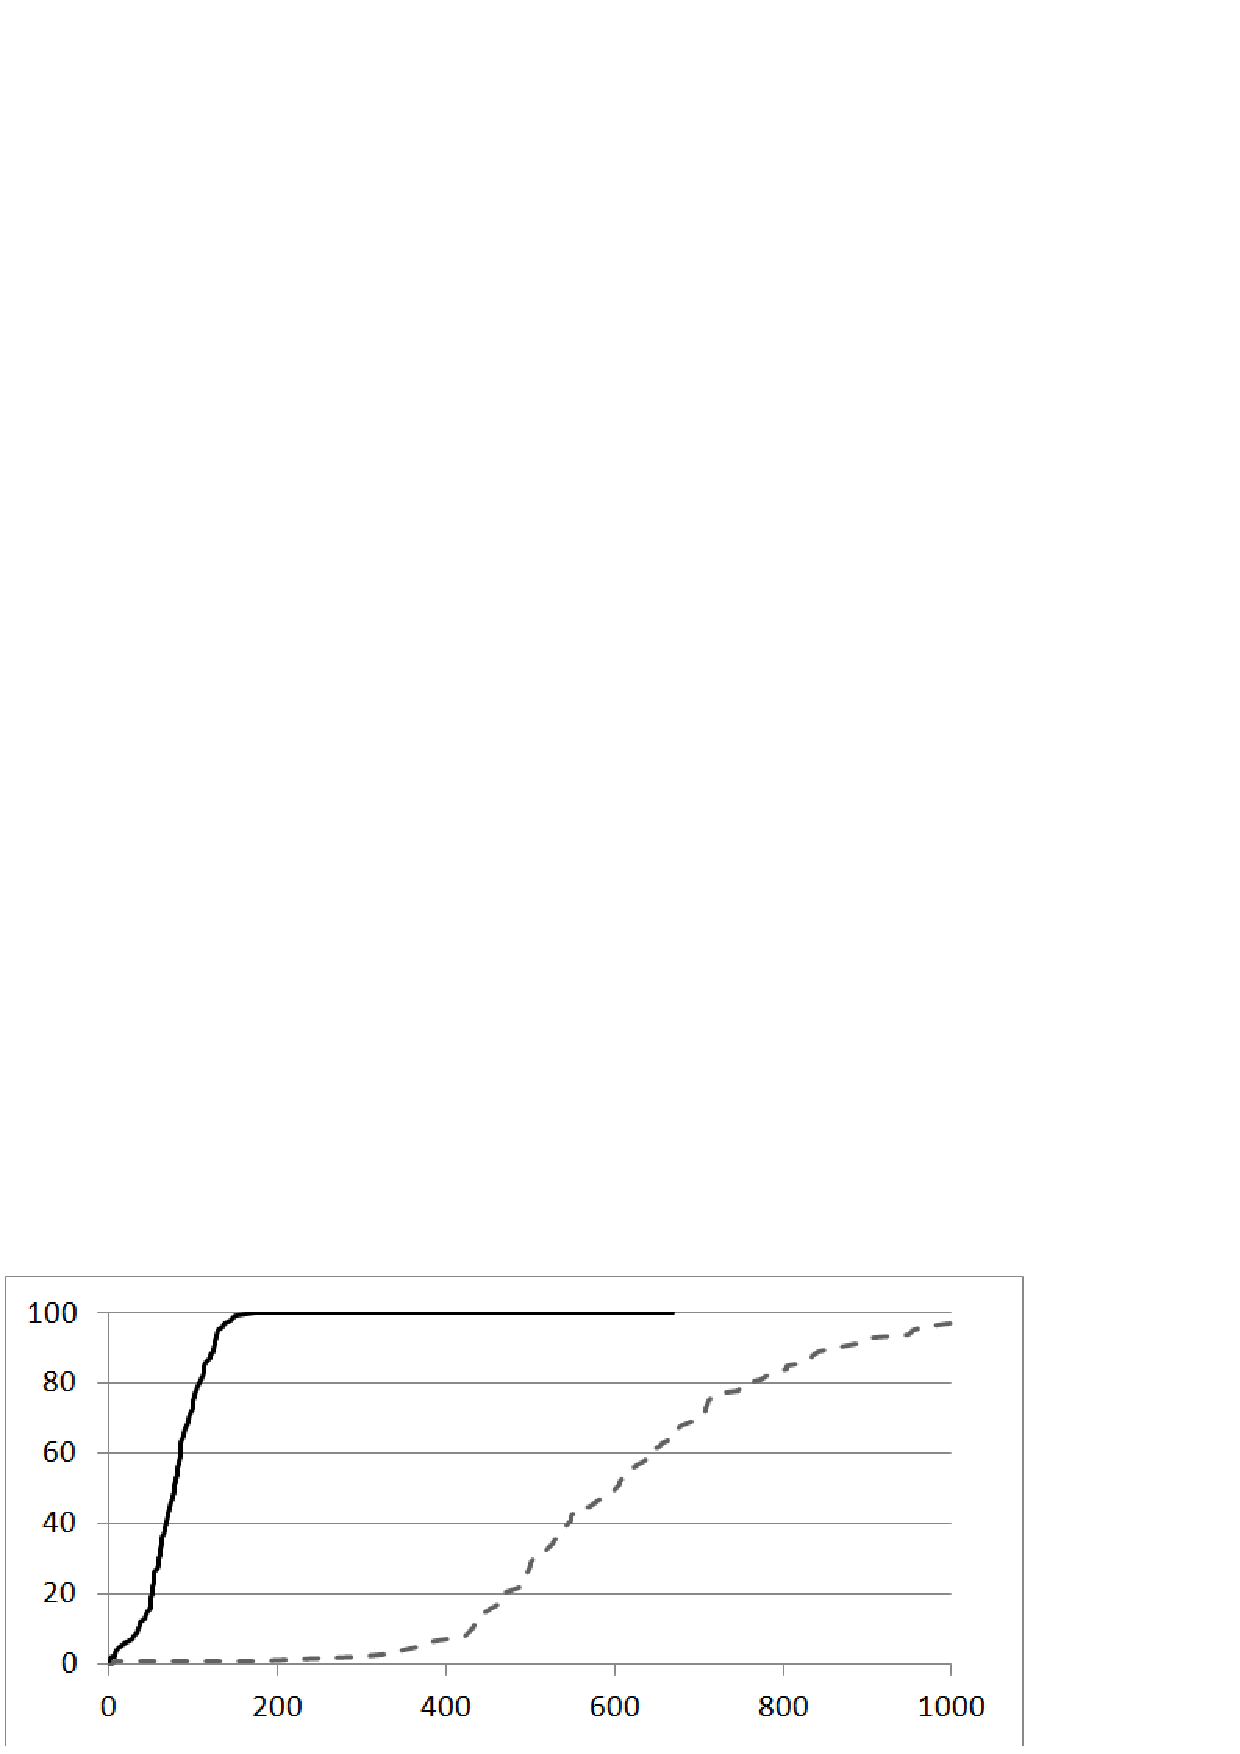
\includegraphics[width=\textwidth]{pic/fig3.png}
\caption{Импутация невычислимых значений средним соседних точек. Подход \No~3} \label{fig3}
\end{figure}

Существенными минусами будет не использование информации о координатах, а также редкость работы добавленного вычислительного правила за счёт поиска значений на замену только среди непосредственных соседей.

\textbf{Четвёртый подход.} Восстанавливать значения целевой функции в точках для интервалов с двумя невычислимыми точками как среднее между ближайшими вычислимыми точками с учётом положения координат, т.е.
\begin{equation}\label{eq17} 
%\tilde{z}(x)=z'+ \text{sign}(z''-z') \frac {|z''-z'| \cdot \| x-x' \|}{\| x''-x' \|},
\tilde{z}(x)=z'+ \text{sign}(z''-z') \frac {|z''-z'| \cdot \rho(x,x')}{\rho(x',x'') },
\end{equation}
где $z'$ и $z''$ -- значения целевой функции в ближайших к интервалу $(x_{i-1},x_i)$ вычислимых точек $x'$ и $x''$, а $\rho(x_1,x_2) =  |x_1 - x_2|^{1/N}$. В остальном подход идентичен третьему. Формула (\ref{eq14}) в данном случае будет применяться лишь тогда, когда невычислимая область находится по соседству с граничной точкой.
\begin{figure}
\centering
\includegraphics[width=\textwidth]{pic/fig4.png}
\caption{Импутация невычислимых значений средним соседних точек. Подход \No~4} \label{fig4}
\end{figure}
\begin{figure}
\centering
\includegraphics[width=\textwidth]{pic/fig5.png}
\caption{Импутация невычислимых значений средним между минорантой и мажорантой. Подход \No~5} \label{fig5}
\end{figure}

\textbf{Пятый подход.} Чтобы максимально использовать поисковую информацию и предположения о виде функции, можно восстанавливать значения целевой функции в точках с учётом условия Гёльдера.

\textit{Шаг 1.} Найти крайние точки пересечения миноранты и мажоранты
\begin{equation}\label{eq18} 
\hat{x}',\hat{x}''=\frac {x'+x''}{2}\pm \text{sign}(z''-z')\cdot \frac {1}{2r} \cdot {\left(\frac {z''-z'}{\mu}\right)}^N,
\end{equation}

\textit{Шаг 2.} Восстановить значения целевой функции по правилу
\begin{equation}\label{eq19} 
\tilde{z}(x)=
  \begin{cases}
    z', & {\quad x \leq \hat{x}',}\\
    %\frac {z'+z''}{2}- \frac {r \mu}{2} (\| x - x' \| + \| x - x'' \|), & {\quad \hat{x}' < x < \hat{x}'',}\\
    \frac {z'+z''}{2}- \frac {r \mu}{2} (\rho(x,x')  + \rho(x,x'')), & {\quad \hat{x}' < x < \hat{x}'',}\\
    z'',  & {\quad x \geq \hat{x}'',}
  \end{cases}
\end{equation}
где $\rho(x_1,x_2) =  |x_1 - x_2|^{1/N}$.
Значение $\tilde{z}(x)$ может быть интерпретировано как среднее значение между минорантой и мажорантой для функции, удовлетворяющей условию Гёльдера.

Приведём описание модификации алгоритма глобального поиска на случай не всюду вычислимой функции на основе данного подхода.

\subsection{Описание модифицированного алгоритма глобального поиска}
Алгоритм остаётся прежним с внесением в него следующих небольших дополнений для вычислительных формул на случай попадания в невычислимые области поиска:

\begin{enumerate}[itemsep=0pt,parsep=2pt,topsep=2pt,partopsep=0pt]
  \item Индекс $v_i=v(x_i)$ определяется по формуле (\ref{eq12}).
  \item При вычислении текущей нижней оценки для константы Гельдера $K$ в формуле (\ref{eq7}) использовать только интервалы с двумя вычислимыми точками.
  \item Текущее лучшее значение целевой функции $z_v^*$ определяется для разных значений индекса
\begin{equation}\label{eq20} 
z_v^*=
  \begin{cases}
    -\varepsilon _r, & {\quad v=0 ,}\\
    \min \left\{ f(x_i): v(x_i)=1, 0 < i < k \right\}, & {\quad v=1 ,}
  \end{cases}
\end{equation}
где $\varepsilon _r > 0$ -- параметр метода.

  \item Для каждого интервала $(x_{i-1}, x_i), 1 \leq i \leq k$, the вычисление характеристики $R(i)$ происходит согласно следующим вычислительным формулам.
      
        \textit{Случай 1.} Для интервалов с \textbf{двумя вычислимыми точками} или \textbf{вычислимой и граничной точками} применить классические правила алгоритма глобального поиска
\begin{equation}\label{eq21} 
R(i)=
  \begin{cases}
     \Delta _i+\frac {{(z_i-z_{i-1})}^2}{{(r \mu)}^2 \Delta _i} - 2 \frac {z_i+z_{i-1}-2z_1^*}{r \mu}, & {\quad  v(x_i)=v(x_{i-1})=1,}\\
    2 \Delta _i-4 \frac {(z_i-z_1^*)}{r \mu}, & {\quad  v(x_{i-1})=-1, v(x_i)=1,}\\
    2 \Delta _i-4 \frac {(z_{i-1}-z_1^*)}{r \mu}, & {\quad  v(x_{i-1})=1, v(x_i)=-1.}
  \end{cases}
\end{equation}
        \textit{Случай 2.} Для интервалов с \textbf{граничной и невычислимой точками} произвести импутацию значения для невычислимой точки на основе соседней вычислимой точки и применить формулу
\begin{equation}\label{eq22} 
R(i)=
  \begin{cases}
    2 \Delta _i-4 \frac {(z_{i+1}-z_0^*)}{r \mu}, & {\quad  v(x_{i-1})=-1, v(x_i)=0,}\\
    2 \Delta _i-4 \frac {(z_{i-2}-z_0^*)}{r \mu}, & {\quad  v(x_{i-1})=0, v(x_i)=-1.}
  \end{cases}
\end{equation}
        \textit{Случай 3.} Для интервалов с \textbf{невычислимой и вычислимой точками} произвести импутацию значения для невычислимой точки на основе соседней вычислимой точки и применить формулу
\begin{equation}\label{eq23} 
R(i)=
  \begin{cases}
     \Delta _i+\frac {{(z_i-z_{i-2})}^2}{{(r \mu)}^2 \Delta _i} - 2 \frac {z_i+z_{i-2}-2z_0^*}{r \mu}, & {\quad  v(x_{i-1})=0, v(x_i)=1,}\\
     \Delta _i+\frac {{(z_{i+1}-z_{i-1})}^2}{{(r \mu)}^2 \Delta _i} - 2 \frac {z_{i+1}+z_{i-1}-2z_0^*}{r \mu}, & {\quad  v(x_{i-1})=1, v(x_i)=0.}
  \end{cases}
\end{equation}
        \textit{Случай 4.} Для интервалов с \textbf{двумя невычислимыми точками} произвести импутацию значений для невычислимой точки на основе правила (\ref{eq19}) и применить формулу
\begin{equation}\label{eq24} 
R(i)=\Delta _i+\frac {{(\tilde{z}_i-\tilde{z}_{i-1})}^2}{{(r \mu)}^2 \Delta _i} - 2 \frac {\tilde{z}_i+\tilde{z}_{i-1}-2z_1^*}{r \mu}, \; v(x_{i-1})=v(x_i)=0.
\end{equation}
        \textit{Случай 5.} В случае невозможности проведения любой импутации использовать формулу
\begin{equation}\label{eq25} 
R(i)=\Delta _i \cdot {\left( 1-\frac {1}{r} \right)}^N+z_0^*.
\end{equation}
  \item Если максимальную характеристику имеют несколько интервалов, отдавать предпочтение вычислимым интервалам с минимальным номером.
  \item Если лучшим интервалом оказался интервал с двумя невычислимыми точками, очередное испытание проводить в серединной точке интервала.
\end{enumerate}

\begin{nmAlgorithm}{pril:prog:alg1}
      {Функция $g$ (вычисление координат точки $v$ по ее порядковому номеру $k$)}
      {Function $g$ (calculating the coordinates of the point $v$ by its ordinal $k$)}
     \algLine{\algFUNC $g(k,d,p)$}
     \algLine[1]{$u_{n-1} \ceq \left\lfloor k/\left(d-1\right)^{n-2}\right\rfloor$}
     \algLine[1]{$u_n \ceq u_{n-1}$}
     \algLine[1]{$k\ceq k\mod (d-1)^{n-2}$}
     \algLine[1]{\algFOR $j=\left(n-3\right)\ldots0$ \algDO}
     \algLine[2]{$u_j\ceq \left\lfloor k/(d-1)^j\right\rfloor+1$}
     \algLine[2]{$k\ceq k\mod(d-1)^j$}
     \algLine[1]{\algENDFOR}
     \algLine[1]{\textbf{return} $(v_1,\dots,v_n)$}
     \algLine{\algENDFUNC}
\end{nmAlgorithm}

\subsection{Условия сходимости}

Установим условия сходимости для модификации алгоритма и покажем, что расширение алгоитма вычисления характеристики не рождает предельных точек другого типа по сравнению с предельными точками классического АГП.

\textbf{Теорема}. Формулировка теоремы.

\textbf{Доказательство}. Доказательство теоремы.

\section{Результаты вычислительных экспериментов}

Вычислительные эксперименты проводились на машине с процессором Intel\textregistered\ Core\texttrademark\ i7-10750H CPU @ 2.60GHz с использованием разработанного программного комплекса, реализующего описанную модификацию из Раздела 3. Для генерации серии задач использовался GKLS-генератор, описанный в [\ref{rfa:rulit:Gaviano2003}]. Он позволяюет порождать задачи многоэкстремальной оптимизации с заранее известными свойствами. Данные задачи были дополнены областями невычислимости разных видов.

Каждая серия экспериментов состоит из 100 задач GKLS со всюду вычислимой целевой функцией (original), 100 задач с невычислимостью на границе области поиска (round) и 100 задач со случайно заданными областями невычислимости (random).

\begin{figure}[h]
\includegraphics[width=\textwidth]{pic/fig6.png}
\caption{Примеры тестовых задач с \No~19, 25, и 35 из первой серии экспериментов} \label{fig6}
\end{figure}

В первой серии экспериментов проверялась корректность работы модификации и выявлялись особенности проведения испытаний в областях невычислимости. В эксперименте использовались задачи размерности $N=2$, параметр надежности был задан $r=5.5$, а точность $\varepsilon=0.01$. Результаты экспериментов представлены в табл.~\ref{tab1}.

На рис.~\ref{fig6} приведены примеры работы модификации с несколькими задачами серии. На рисунках синими точками отмечены испытания в вычислимых областях, красным найденный глобальный минимум задачи, а черным -- точки испытаний, проводившихся в области невычислимости. Также для наглядности области невычислимости окрашены в серый цвет.

Так как модификация с классической серией задач GKLS работает согласно базовому алгоритму глобального поиска, можно провести ее сравнение с классическим АГП. Так, для модификации сохранено общее поведение АГП и наблюдаются те же области сгущения испытаний вблизи локальных минимумов, что объясняется срабатыванием в большинстве случаев именно классических вычислительных правил (\ref{eq21}), в табл.~\ref{tab1} видно, что число испытаний, проводимых в невычислимых областях не велико. Общее число испытаний для классических задач и задач с невычислимостями соизмеримо, метод не проводит избыточных итераций в неперспективных областях благодаря расчётным формулам, использующим информацию о ближайших вычислимых точках. 

\begin{table}[h]
\caption{Сравнение модификации алгоритма с классической версией алгоритма глобального поиска}\label{tab1}
\centering
\begin{tabular}{|l|c|c|c|}
\hline
 &  { original }  & { round }  & { random }  \\
\hline
Среднее число испытаний & 781.7	& 854.9 & 839.0 \\
\begin{tabular}{@{}l@{}} {Среднее число испытаний} \\  { в областях невычислимости } \end{tabular}  & - & 185.8 & 42.3 \\
{Число решенных задач} & 100 / 100 & 100 / 100  &  100 / 100 \\
\hline
\end{tabular}
\end{table}

Использование правила (\ref{eq25}) формирует сетку испытаний внутри граничных областей невычислимости, что хорошо заметно на задаче \No~35. При этом у границы невычислимой области близкой к потенциальному минимума формируется сгущение точек испытаний при попытке подойти к нему с разных сторон благодаря вычислительным правилам (\ref{eq22})--(\ref{eq24}), что наблюдается во всех приведенных в качестве примеров задачах. 

Решаемость задач 100\%, однако для серии с граничной областью потребо-валось дорешивание одной задачи с немного большим значением $r=6.0$, для серии со случайными областями то же значение $r$ использовалось для решения двух задач.

\begin{table}
\caption{Серия задач разной размерности}\label{tab2}
\centering
\begin{tabular}{|l|l|c|c|c|}
\hline
 \begin{tabular}{@{}c@{}} {N} \\ {}\end{tabular} &
 \begin{tabular}{@{}c@{}} {Тип} \\ {тестовых задач} \end{tabular} &
 \begin{tabular}{@{}c@{}} {Среднее число испытаний} \\ {} \end{tabular} &
 \begin{tabular}{@{}c@{}} {Среднее число испытаний} \\ {в области невычислимости} \end{tabular} &
 \begin{tabular}{@{}c@{}} {Число решенных задач} \\ {}\end{tabular} \\
\hline
$3$ & original & 12251.1 & - & 100 / 100 \\
$ $ & round & 12201.8 & 4763.6 & 100 / 100 \\
$ $ & random & 12210.7 & 63.4 & 100 / 100 \\
\hline
$4$ & original & 25144.5 & - & 100 / 100 \\
$ $ & round & 29840.3 & 15004.4  & 100 / 100 \\
$ $ & random & 25287.5 & 26.4 & 100 / 100 \\
\hline
$5$ & original & 56725.9 & - & 100 / 100 \\
$ $ & round & 47840.1 & 24109.2 & 100 / 100\\
$ $ & random & 57874.8 & 82.6 & 100 / 100\\
\hline
\end{tabular}
\end{table}

Во второй серии экспериментов проводилось решение серий задач разных размерностей. В эксперименте использовались задачи размерности $N=3,4,5$, параметр надежности был задан $r=4.5$, а точность $\varepsilon=0.02$. Глобальный минимум считался найденным, если алгоритм генерировал точку испытания в $\varepsilon$-окрестности глобального минимума. Результаты выполненных экспериментов представлены в табл.~\ref{tab2}.

Как показывают результаты выполненных экспериментов, метод отлично справляется со случайными попаданиями в области невычислимости, разбросанными по области поиска случайно, а в случае больших граничных областей пытается провести полноценное исследование, не проводя при этом слишком много испытаний.

\section{Заключение}

В данной работе была рассмотрена задача нахождения глобального минимума дорогостоящей липшицевой функции вида ``черный ящик''. По сравнению с традиционной формулировкой, используемой в глобальной оптимизации, задача рассмотренная здесь имеет важное отличие: целевая функция может быть не определена в некоторых подобластях области поиска (в частном случае, в одной или нескольких ее точках). В таких подобластях невозможно корректно провести численное моделирование и вычислить значение целевой функции. Появление данной постановки обусловлено частой проблемой численной нестабильности исследуемых моделей прикладных задач.

Основная трудность заключается в невозможности в большинстве случаев заранее узнать о подобластях невычислимости, фактически, область допустимых сочетаний параметров является заранее неопределенной. Данное явление можно интерпретировать либо как наличие в задаче некоторых скрытых ограничений.

Исследуемая в данной работе проблема является частичным аналогом уже давно существующей в Data Science проблемы пропущенных значений. В качестве решения специалистами в данной сфере были предложены различные подходы к импутации (восстановлению) пропущенных значений. %Эти идеи нашли своё отражение при разработке нового метода.

Было проведено исследование применимости уже существующих подходов, дополненных различными вариантами учета липшицевости функции и использующих информационно-статистическую теорию. В результате удалось разработать универсальный эффективный алгоритм для данного класса задач. Построенный алгоритм является развитием одного из эффективных детерминированных методов решения задач липшицевой глобальной оптимизации – информационно-статистического алгоритма глобального поиска. В рамках модификации была произведена адаптация вычислительных правил алгоритма с внедрением алгоритма импутации значений.

Были проведены численные эксперименты на сериях многоэкстремальных задач GKLS размерностей $N = 2,3,4,5$. Результаты продемонстрировали надежность и эффективность предложенного подхода. Модификация отлично справляется со случайными попаданиями в подобласти невычислимости, разбросанными по области поиска. В случае больших граничных областей невычислимости метод всё также эффективно решает задачу, проводя полноценное исследование, в том числе, в невычислимых областях.

%=======================  Список литературы ==================================
%
% Команда \LITERRUS печатает "СПИСОК ЛИТЕРАТУРЫ" и обнуляет счетчики
%
\LITERRUS
% \rlitem{arg1}{arg2} --- создает пункт списка литературы.
% arg1 --- символическая ссылка на источник, используется при создании ссылки командой \ref
% arg2 --- текст, помещаемый в пункт списка. Может содержать команды выбора начертания 
%          символов и др.

%7
\rlitem{rfa:rulit:Grishagin2016_2}{%
\textit{Grishagin~V.A., Israfilov~R.A.}
Global search acceleration in the nested optimization scheme~// 
AIP Conference Proceedings. 2016. \textbf{1738}. 400010.
\doi{10.1063/1.4952198}.
}
%9
\rlitem{rfa:rulit:Jones2021}{%
\textit{Jones~D., Martins~J.}
The direct algorithm: 25 years later~// 
J. Glob. Optim. 2021. \textbf{79}, N~3. 521--566.
\doi{10.1007/s10898-020-00952-6}.
}
%12
\rlitem{rfa:rulit:PaulaviciusZilinskas2014}{%
\textit{Paulavi{\v c}ius~R. and {\v Z}ilinskas~J.}
Simplicial Global Optimization.
New York: Springer, 2014.
\doi{10.1007/978-1-4614-9093-7}.
}
%13
\rlitem{rfa:rulit:Birect2020}{%
\textit{Paulavi{\v c}ius~R., Sergeyev~Y.D., Kvasov~D.E., {\v Z}ilinskas~J.}
Globally-biased {BIRECT} algorithm with local accelerators for expensive global optimization~// 
Expert Syst. Appl. 2020. \textbf{144}. 113052.
\doi{10.1016/j.eswa.2019.113052}.
}
%14
\rlitem{rfa:rulit:Sergeyev2017}{%
\textit{Sergeyev~Y.D., Kvasov~D.E.}
Deterministic global optimization: An introduction to the diagonal approach.
New York: Springer, 2017.
\doi{10.1007/978-1-4939-7199-2}.
}
%11
\rlitem{rfa:rulit:Liberti2005}{%
\textit{Liberti~L., Kucherenko~S.}
Comparison of deterministic and stochastic approaches to global optimization~// 
Int. Trans. Oper. Res. 2005. \textbf{12}. 263--285.
}
%15
\rlitem{rfa:rulit:Sergeyev2018}{%
\textit{Sergeyev~Y.D., Kvasov~D.E., Mukhametzhanov~M.S.}
On the efficiency of nature-inspired metaheuristics in expensive global optimization with limited budget~// 
Sci. Rep. 2018. \textbf{8}, N~1. 435.
}
%16
\rlitem{rfa:rulit:Sergeyev2013}{%
\textit{Sergeyev~Y.D., Strongin~R.G., Lera~D.}
Introduction to Global Optimization Exploiting Space-Filling Curves.
New York: Springer Briefs in Optimization, 2013.
\doi{10.1007/978-1-4614-8042-6}.
}
%20
\rlitem{rfa:rulit:Strongin2000}{%
\textit{Strongin~R.G., Sergeyev~Y.D.}
Global optimization with non-convex constraints. Sequential and parallel algorithms.
Dordrecht: Kluwer Academic Publishers, 2000.
}
%10
\rlitem{rfa:rulit:Kvasov2013}{%
\textit{Kvasov~D.E., Sergeyev~Y.D.}
Lipschitz global optimization methods in control problems~// 
Autom. Remote Control. 2013. \textbf{74}, N~9. 1435--1448.
\doi{10.1134/s0005117913090014}.
}
%17
\rlitem{rfa:rulit:Sergeyev2020}{%
\textit{Sergeyev~Y.D., Candelieri~A., Kvasov~D.E., Perego~R.}
Safe global optimization of expensive noisy black-box functions in the $\delta$-Lipschitz framework~// 
Soft Comput. 2020. \textbf{24}, N~23. 17715--17735.
\doi{10.1007/s00500-020-05030-3}.
}
%4
\rlitem{rfa:rulit:Dongarra2022}{%
\textit{Dongarra~J.J.}
The evolution of mathematical software~// 
Commun. ACM. 2022. \textbf{65}, N~12. 66--72.
\doi{10.1145/3554977}.
}
%5
\rlitem{rfa:rulit:Duwe2020}{%
\textit{Duwe~K., et al.}
State of the art and future trends in data reduction for high-performance computing~// 
Supercomput. Front. Innov. 2020. \textbf{7}, N~1.
\doi{10.14529/jsfi200101}.
}
%19
\rlitem{rfa:rulit:Stripinis2021}{%
\textit{Stripinis~L., Paulavi{\v c}ius~R.}
A new {DIRECT}-{GLh} algorithm for global optimization with hidden constraints~// 
Optim. Lett. 2021. \textbf{15}, N~6. 1865--1884.
\doi{10.1007/s11590-021-01726-z}.
}
%1
\rlitem{rfa:rulit:Audet2022}{%
\textit{Audet~C., Batailly~A., Kojtych~S.}
Escaping unknown discontinuous regions in blackbox optimization~// 
SIAM J. Optim. 2022. \textbf{32}, N~3. 1843--1870.
\doi{10.1137/21m1420915}.
}
%3
\rlitem{rfa:rulit:Candelieri2019}{%
\textit{Candelieri~A.}
Sequential model based optimization of partially defined functions
under unknown constraints~// 
J. Glob. Optim. 2019. \textbf{79}, N~2. 281--303.
\doi{10.1007/s10898-019-00860-4}.
}
%18
\rlitem{rfa:rulit:Sergeyev2003}{%
\textit{Sergeyev~Y.D., Pugliese~P., Famularo~D.}
Index information algorithm with local tuning for solving multidimensional global optimization problems with multiextremal constraints~// 
Math. Program. 2003. \textbf{96}, N~23. 489--512.
\doi{10.1007/s10107-003-0372-z}.
}
%21
\rlitem{rfa:rulit:Strongin2020}{%
\textit{Strongin~R.G., Barkalov~K.A., Bevzuk~S.A.}
Global optimization method with dual Lipschitz constant estimates for problems with non-convex constraints~// 
Soft Comput. 2020. \textbf{24}, N~16. 11853--11865.
\doi{10.1007/s00500-020-05078-1}.
}
%2
\rlitem{rfa:rulit:Barkalov2022}{%
\textit{Barkalov~K.A., et al.}
On solving the problem of finding kinetic parameters of catalytic isomerization of the pentane-hexane fraction using a parallel global search algorithm~// 
Mathematics. 2022. \textbf{10}, N~19. 3665.
\doi{10.3390/math10193665}.
}
%8
\rlitem{rfa:rulit:Gubaydullin2022}{%
\textit{Gubaydullin~I.M., Enikeeva~L.V., Barkalov~K.A., Lebedev~I.G., Silenko~D.G.}
Kinetic modeling of isobutane alkylation with mixed c4 olefins and sulfuric acid as a catalyst using the asynchronous global optimization algorithm~// 
Commun. Comput. Inf. Sci. 2022. \textbf{1618}. 293--306.
\doi{10.1007/978-3-031-11623-0_20}.
}
%6
\rlitem{rfa:rulit:Gaviano2003}{%
\textit{Gaviano~M., Kvasov~D.E., Lera~D., Sergeyev~Y.D.}
Software for generation of classes of test functions with known local and global minima for global optimization~// 
ACM Trans. Math. Softw. 2003. \textbf{29}, N~4. 469--480.
}

%=======================  Список литературы ==================================
\medskip
\DateRU 

\medskip

\MakeAuthorsInfoRU

%===========================  REFERENCES =====================================
\pagebreak

\REFERENCES

%7
\elitem{rfa:enlit:Grishagin2016_2}{%
V.~A.~Grishagin, R.~A.~Israfilov, ``Global search acceleration in the nested optimization scheme'',
AIP Conference Proceedings. {\bf 1738}, 400010 (2016). 
\doi{10.1063/1.4952198}.
}
%9
\elitem{rfa:enlit:Jones2021}{%
D.~Jones, J.~Martins, ``The direct algorithm: 25 years later'',
J. Glob. Optim. {\bf 79} (3), 521--566 (2021). 
\doi{10.1007/s10898-020-00952-6}.
}
%12
\elitem{rfa:enlit:PaulaviciusZilinskas2014}{%
R.~Paulavi{\v c}ius and J.~{\v Z}ilinskas
{\it Simplicial Global Optimization}
(Springer, New York, 2014).
\doi{10.1007/978-1-4614-9093-7}.
}
%13
\elitem{rfa:enlit:Birect2020}{%
R.~Paulavi{\v c}ius, Y.~D.~Sergeyev, D.~E.~Kvasov, J.~{\v Z}ilinskas, ``Globally-biased {BIRECT} algorithm with local accelerators for expensive global optimization'', 
Expert Syst. Appl. {\bf 144}, 113052 (2020).
\doi{10.1016/j.eswa.2019.113052}.
}
%14
\elitem{rfa:enlit:Sergeyev2017}{%
Y.~D.~Sergeyev, D.~E.~Kvasov
{\it Deterministic global optimization: An introduction to the diagonal approach}
(Springer, New York, 2017).
\doi{10.1007/978-1-4939-7199-2}.
}
%11
\elitem{rfa:enlit:Liberti2005}{%
L.~Liberti, S.~Kucherenko, ``Comparison of deterministic and stochastic approaches to global optimization'',
Int. Trans. Oper. Res. {\bf 12}, 263--285 (2005).
}
%15
\elitem{rfa:enlit:Sergeyev2018}{%
Y.~D.~Sergeyev, D.~E.~Kvasov, M.~S.~Mukhametzhanov, ``On the efficiency of nature-inspired metaheuristics in expensive global optimization with limited budget'',
Sci. Rep. {\bf 8} (1), 435 (2018).
}
%16
\elitem{rfa:enlit:Sergeyev2013}{%
Y.~D.~Sergeyev, R.~G.~Strongin, D.~Lera
{\it Introduction to Global Optimization Exploiting Space-Filling Curves}
(Springer Briefs in Optimization, Springer, New York, 2013).
\doi{10.1007/978-1-4614-8042-6}.
}
%20
\elitem{rfa:enlit:Strongin2000}{%
R.~G.~Strongin, Y.~D.~Sergeyev
{\it Global optimization with non-convex constraints. Sequential and parallel algorithms}
(Kluwer Academic Publishers, Dordrecht, 2000).
}
%10
\elitem{rfa:enlit:Kvasov2013}{%
D.~E.~Kvasov, Y.~D.~Sergeyev, ``Lipschitz global optimization methods in control problems'',
Autom. Remote Control. {\bf 74} (9), 1435--1448 (2013).
\doi{10.1134/s0005117913090014}.
}
%17
\elitem{rfa:enlit:Sergeyev2020}{%
Y.~D.~Sergeyev, A.~Candelieri, D.~E.~Kvasov, R.~Perego, ``Safe global optimization of expensive noisy black-box functions in the $\delta$-Lipschitz framework'',
Soft Comput. {\bf 24} (23), 17715--17735 (2020).
\doi{10.1007/s00500-020-05030-3}.
}
%4
\elitem{rfa:enlit:Dongarra2022}{%
J.~J.~Dongarra, ``The evolution of mathematical software'', 
Commun. ACM. {\bf 65} (12), 66--72 (2022).
\doi{10.1145/3554977}.
}
%5
\elitem{rfa:enlit:Duwe2020}{%
K.~Duwe, et al., ``State of the art and future trends in data reduction for high-performance computing'',
Supercomput. Front. Innov. {\bf 7} (1), (2020).
\doi{10.14529/jsfi200101}.
}
%19
\elitem{rfa:enlit:Stripinis2021}{%
L.~Stripinis, R.~Paulavi{\v c}ius, ``A new {DIRECT}-{GLh} algorithm for global optimization with hidden constraints'',
Optim. Lett. {\bf 15} (6), 1865--1884 (2021).
\doi{10.1007/s11590-021-01726-z}.
}
%1
\elitem{rfa:enlit:Audet2022}{%
Audet~C., Batailly~A., Kojtych~S., ``Escaping unknown discontinuous regions in blackbox optimization'',
SIAM J. Optim. {\bf 32} (3), 1843--1870 (2022).
\doi{10.1137/21m1420915}.
}
%3
\elitem{rfa:enlit:Candelieri2019}{%
A.~Candelieri, ``Sequential model based optimization of partially defined functions under unknown constraints'',
J. Glob. Optim. {\bf 79} (2), 281--303 (2019).
\doi{10.1007/s10898-019-00860-4}.
}
%18
\elitem{rfa:enlit:Sergeyev2003}{%
Y.~D.~Sergeyev, P.~Pugliese, D.~Famularo, ``Index information algorithm with local tuning for solving multidimensional global optimization problems with multiextremal constraints'', 
Math. Program. {\bf 96} (23), 489--512 (2003).
\doi{10.1007/s10107-003-0372-z}.
}
%21
\elitem{rfa:enlit:Strongin2020}{%
R.~G.~Strongin, K.~A.~Barkalov, S.~A.~Bevzuk, ``Global optimization method with dual Lipschitz constant estimates for problems with non-convex constraints'',
Soft Comput. {\bf 24} (16), 11853--11865 (2020).
\doi{10.1007/s00500-020-05078-1}.
}
%2
\elitem{rfa:enlit:Barkalov2022}{%
K.~A.~Barkalov, et al., ``On solving the problem of finding kinetic parameters of catalytic isomerization of the pentane-hexane fraction using a parallel global search algorithm'',
Mathematics. {\bf 10} (19), 3665 (2022).
\doi{10.3390/math10193665}.
}
%8
\elitem{rfa:enlit:Gubaydullin2022}{%
I.~M.~Gubaydullin, L.~V.~Enikeeva, K.~A.~Barkalov, I.~G.~Lebedev, D.~G.~Silenko, ``Kinetic modeling of isobutane alkylation with mixed c4 olefins and sulfuric acid as a catalyst using the asynchronous global optimization algorithm'',
Commun. Comput. Inf. Sci. {\bf 1618}, 293--306 (2022).
\doi{10.1007/978-3-031-11623-0_20}
}
%6
\elitem{rfa:enlit:Gaviano2003}{%
M.~Gaviano, D.~E.~Kvasov, D.~Lera, Y.~D.~Sergeyev, ``Software for generation of classes of test functions with known local and global minima for global optimization'',
ACM Trans. Math. Softw. {\bf 29} (4), 469--480 (2003).
}

\medskip
\DateEN

\bigskip

\MakeAuthorsInfoEN

%\end{document}
%============================ КОНЕЦ СТАТЬИ ==================================


%%%%%%%% В КОНЦЕ УДАЛИТЬ

%\section{Рекомендации к содержанию и структуре статей}

%Авторам оригинальных статей рекомендуется объем до 20 страниц.

%Объем аннотации не должен превышать 10--15 строк. Разбивать аннотации на абзацы не рекомендуется.

%Авторы статьи указывают УДК (для статей на русском языке), которым соответствует публикация.

%Рекомендуется для лучшего восприятия разбивать текст на абзацы размером не более 10--15~строк.

%Список литературы является неотъемлемой частью статьи и оформляется непосредственно в тексте статьи: использование отдельных файлов с расширениями bib, bbl и других не допускается. 

%Авторы статей, публикуемых в журнале на русском языке, должны предоставить переведенные на английский язык:
%\begin{itemize}[itemsep=0pt,parsep=0pt,topsep=0pt,partopsep=0pt]
%\item фамилию, имя, отчество, ученую степень, ученое звание и должность каждого автора;
%\item название, почтовые адреса организаций, являющихся основными местами работы авторов, и их должности в этих организациях;
%\item название статьи;
%\item текст аннотации;
%\item ключевые слова;
%\item слова благодарности;
%\item подписи к рисункам, таблицам, листингам программ и алгоритмов, а также всю текстовую информацию, содержащуюся на рисунках, в таблицах и пр.
%\end{itemize}
%\vspace*{2mm}


%Между инициалами и фамилией всегда должен ставится пробел (А.А.~Иванов).
%В заголовке статьи пробелы также ставятся между инициалами: А.~А.~Иванов.

%Точка не ставится после заголовков разделов, названий таблиц и подписей рисунков, после ряда сокращенных наименований: с~--- секунда, г~--- грамм, мин~--- минута, сут~--- сутки, млн~--- миллион, млрд~--- миллиард и т.п. Точка ставится в конце последнего предложения аннотации, в конце списка ключевых слов, после сокращений: мес.~--- месяц, г.~--- год и др.

%Для набора выключных формул рекомендуется использовать окружение {\tt equation} с автоматической сквозной нумерацией. Для подавления нумерации используйте окружение {\tt equation*}.

%\pagebreak
%\smallskip

%\item Слова ``Теорема'', ``Следствие'', ``Лемма'', ``Утверждение'', ``Предложение'' помещаются в текст статьи явно и выделяются прямым полужирным шрифтом, а соответствующие формулировки печатаются прямым шрифтом.
%\item Слова ``Доказательство'', ``Определение'', ``Примечание'', ``Замечание'' выделяются прямым полужирным шрифтом, а соответствующие формулировки печатаются прямым шрифтом.
%\item Рекомендуется выполнять сквозную нумерацию арабскими цифрами для теорем, %лемм, определений и т.д. 

%Допускается воспроизводить небольшие по объему (рекомендуется не более 1 страницы) фрагменты программ, иллюстрирующие важные для понимания статьи алгоритмы, средства языков программирования и т.п. Текстовые сообщения и комментарии в листингах должны быть представлены на английском языке.

%Рекомендуются следующие размеры иллюстраций: а)~шириной не более 165~мм и высотой не более 210~мм (в ширину колонки текста); б)~шириной не более 80 мм и высотой не более 140~мм (в половину ширины колонки); в) высотой 145~мм и шириной 240~мм (иллюстрация, развернутая на $90^\circ$ на всю страницу).
%Принимаются иллюстрации трех видов: штриховые рисунки (графики, диаграммы, графы и пр.), скриншоты экрана компьютера (например, цветовая визуализация поля, полученная в результате математического моделирования) и фотографии.
%Штриховые рисунки принимаются в виде файлов формата PNG (растр) разрешением 600 DPI при масштабе рисунка 1:1 или в формате EPS (векторные рисунки). Толщина самой тонкой линии на рисунке не должна быть меньше 5~px. Рекомендуется для основных линий использовать черный цвет. Важные для понимания элементы рисунка должны выделяться двумя-тремя цветами, которые контрастно воспроизводятся при черно-белой печати. Цвет фона рекомендуется белый. Фотографии принимаются в форматах JPEG, PNG, TIFF разрешением 300 DPI. Изображение на фотографии должно быть резким, контрастным. Цифровая обработка изображения не должна вызывать сомнений в достоверности фотографии. Надписи на рисунках должны быть выполнены на английском языке. Рекомендуется важные элементы рисунка обозначать цифрами и давать расшифровку в подписи. Серия иллюстраций предназначается для сравнения графиков, оценки влияния параметров, объяснения трендов, динамики и т.п. Рисунки, входящие в серию, должны быть одинакового размера и разрешения. Каждая иллюстрация в серии должна быть обозначена буквой английского алфавита.
%Редакция просит предоставлять наряду с файлами EPS исходные, необработанные файлы в форматах TIFF, PNG, JPEG. 
    
%Подписи к рисункам, заголовки таблиц, листингов программ и алгоритмов должны быть выполнены на русском и английском языках. Для этого в стилевом файле определены команды \verb!\bicaption!.

%Список литературы формируется в порядке обращения к источникам в       тексте статьи.

%Для уменьшения вероятности ошибок в ссылках по тексту статьи необходимо пользоваться командами \verb!\label!, автоматически сохраняющей значения счетчиков для рисунков, таблиц, списков в символической переменной, и \verb!\ref!, которая создает ссылку по имени переменной.

%Необходимые документы
%Для публикации статьи авторы должны предоставить: 
% сопроводительное письмо авторов (Приложение~1 в этом документе) в электронном виде и его отсканированный вариант с ``живыми'' подписями;
% электронную \LaTeX--версию статьи (на русском или/и английском языках), подготовленную в соответствии с требованиями к оформлению статей, а также pdf--файл статьи и рисунки;
% текстовый файл, содержащий следующую информацию на русском и английском языках: а)~фамилия, имя, отчество, ученая степень, ученое звание, ORCID и e-mail каждого из авторов; б)~названия и почтовые адреса организаций, являющихся основными местами работы авторов и их должности в этих организациях; в)~название статьи; г)~текст аннотации; д)~ключевые слова.
%Автор взаимодействует с редакцией в основном через сайт журнала \url{https://num-meth.ru}. После заполнения регистрационной формы автор (один из авторов) должен:
%\item загрузить через форму все подготовленные необходимые документы и компоненты статьи в виде ZIP--архива, выбрав при загрузке {\tt Компонент статьи = ``ZIP-архив с исходными текстами (.tex и требуемые дополнительные файлы)''};
%\item дать описание архива, авторство и т.п. (рекомендуется сделать на этапе проверки деталей отправляемого файла);
%\item подтвердить отправку архива;
%\item ввести метаданные статьи (обязательно заголовок, аннотацию и ключевые слова) и информацию об авторе и всех соавторах (вся информация должна заноситься на русском и дублироваться на английском языке);
%\item подтвердить внесенные данные.

%%%%%%%% В КОНЦЕ УДАЛИТЬ

%============================ ПРИЛОЖЕНИЕ 6 ==================================
\newpage\nolinenumbers
%
% ПРИЛОЖЕНИЕ 4
% используйте как шаблон письма в редакцию
%
\thispagestyle{empty}
%
% Следующие две строки нужно убрать
%
%\appendix{Сопроводительное письмо в редакцию}{pril:sopr}
%

{\large
\hfill\parbox[t]{80mm}{
Главному редактору научного журнала\\[2mm]
``Вычислительные методы и\\
программирование''\\[2mm]
чл.-корр. РАН, проф. Вл. В. Воеводину
}
\vspace*{12mm}
\begin{center}
СОПРОВОДИТЕЛЬНОЕ ПИСЬМО
\end{center}

\vspace*{3mm}

Просим опубликовать в журнале ``Вычислительные методы и программирование'' статью 
``<НАЗВАНИЕ СТАТЬИ>''.

Сообщаем следующую информацию о каждом авторе статьи.

1. Фамилия, имя, отчество полностью (с написанием на английском языке).

2. Основное место работы полностью с указанием полного почтового адреса и URL сайта организации (с переводом на английский язык).

3. Должность по основному месту работы (с переводом на английский язык).

4. Ученая степень и ученое звание (с переводом на английский язык).

5. Телефон служебный, домашний и мобильный.

6. E-mail.

7. ORCID (\corr{обязательно}; если еще не получен, посетите \url{https://orcid.org/register}).

8. Номер и название рубрики ГРНТИ (только для статей на русском) и код OECD для подаваемой статьи.

9. Желательно: ссылки на профили авторов в elibrary.ru для упрощения и корректности подлинковки статьи.

\vspace*{2mm}
Текущую переписку по вопросам публикации статьи следует вести с <Фамилия И.О.>.

\vspace*{2mm}
Авторы согласны с правилами подготовки статьи к публикации, включая рецензирование, 
научное и литературное редактирование и доведение статьи до редакторских стандартов, 
принятых в рамках журнала.

Авторы ознакомлены с Публикационной этикой журнала и согласны с ее положениями.

Авторы также согласны с передачей журналу своего права на издание и распространение 
статьи в электронной и бумажной версиях, в том числе на размещение библиографической 
информации о статье в Российском индексе научного цитирования (РИНЦ) и в других базах 
научного цитирования и на размещение полных текстов статей в Научной электронной 
библиотеке (elibrary.ru) и портале http://www.mathnet.ru для свободного доступа всем пользователям Интернет независимо от их категории и местоположения.

\vspace*{15mm}
<Дата>\hfill\parbox[t]{70mm}{\hrulefill~<И.О. Фамилия>}

\vspace*{8mm}

\hfill\parbox[t]{70mm}{\hrulefill~<И.О. Фамилия>}

}%large

\end{document}

